\section{Experiments}
\label{seq:results}

In this section, we present extensive experiments to evaluate our proposal. We consider two localisation scenarios: indoor static scenes (section~\ref{subseq:indoor}) and outdoor dynamic scenes (section~\ref{subseq:outdoor}). We also divide our evaluation according to the data available to train our encoder/decoder architecture: fully supervised depth from monocular training (when ground-truth associated depth map are available during training), and unsupervised depth from monocular (when the only data available during training are video sequences with relative poses between images).

\subsection{Implementation details}
\label{subseq:implementation}

\paragraph{Datasets.} We test our method on the following indoor localisation datasets: 7 scenes~\citep{Shotton2013} and 12 scenes~\citep{Valentin2016}. These datasets are composed of various indoor environments scanned with RGB-D sensors. We use the Cambridge Landmarks~\citep{Kendall2015} dataset for outdoor evaluation. This dataset is composed of 6 scenes featuring dynamic changes (pedestrian and cars in movement during the acquisition) acquired by a cell-phone camera. 6-DoF image poses and camera calibration parameters are provided for these 3 datasets. For all the experiments, reference images used for the initial pose estimation with CBIR are taken from the training split and query images are taken from the testing split of the respective datasets.

As not ground truth depth maps are available for the Cambridge Landmarks scenes, we only perform outdoor experiments related to the unsupervised depth from monocular training.

\paragraph{Networks architecture and training.} For both fully supervised and unsupervised depth from monocular experiments, we use a U-Net like convolutional encoder/decoder architecture~\citep{Isola2017} with multi-scale outputs~\citep{Godard2017}. For the unsupervised scenario, we also try to add some recurrent layers (LSTM) in the decoder to capture long term dependencies~\citep{Visin2015, Li2016b}. We denote the fully convolutional architecture as \textbf{FC} and convolutional layers + recurrent layers architecture as \textbf{C+LSTM}. FC and C+LSTM encoders are identical, with 6.3M parameters, FC decoder has 16.7M parameters and C+LSTM decoder has 10.1M parameters.

During training and testing, images are resized to $224 \times 224$ pixels for indoor scenes, and $224 \times 112$ for outdoor images. The generated depth map is 4 times smaller than the RGB input. We use $L_1$ loss function for the fully supervised depth from monocular training. To learn depth from RGB in a unsupervised manner, we follow the training procedure of~\citep{Zhou2017a}, using the ground truth relative pose between images and by adding SSIM loss function for radiometric comparison as in~\citep{Mahjourian2018}. We train all the architecture with adam optimizer, learning rate of $10^{-4}$ divided by two every 50, respectively 5, epochs for the supervised, respectively unsupervised, training. Training takes approximately one day on our Nvidia Titan X GPU with a batch size is set to 24, respectively 12, for supervised, respectively unsupervised, training.

We train networks for indoor localisation on the 7 scenes dataset (using only sequences from the training split). The 12 scenes dataset is used to evaluate the generalisation capability of our method. For outdoor localisation, we train our two different architectures (FC and C+LSTM) on the Cambridge Landmarks dataset.

\paragraph{Method parameters.} We use NetVLAD layer with 64 clusters as global image descriptor for initial pose estimation. We concatenate features from the last convolutional layers of the encoder network, composed of 256 convolutional filters, resulting in a global descriptor of size 16384. Descriptor dimension can be further reduced with PCA projection~\citep{Arandjelovic2017}. We consider the 5-top retrieved candidates from the nearest neighbour search in the pose refinement process, resulting in a good trade-off between time consumption and pose estimation performances. For the final pose estimation, we use the fast \texttt{C++} PnP implementation from~\citep{Kneip2014opengv} and we set the inlier ratio threshold mentioned in section~\ref{subsec:pnlp} to 10\%.
% Local feature for the dense matching between query image and retrieved candidates are extracted from the second convolutional layer of the encoder, resulting on 64-dimensions local descriptors.

\subsection{Indoor localisation}
\label{subseq:indoor}

\begin{table}
\centering

\begin{footnotesize}
\renewcommand{\arraystretch}{1.0}
\newcolumntype{Y}{>{\centering\arraybackslash}X}
\begin{tabular}{c l | c c | c c | c c }
					&		&	\multicolumn{2}{c|}{\textit{Image retrieval}} & \multicolumn{2}{c|}{PnlP refinement} & Relocnet & Posenet  \\
	\multicolumn{2}{c|}{Scene} 	&	 \purple{FC-sup.}	  & \blue{FC-unsup.} & \purple{FC-sup.}	& \blue{FC-unsup.}  & \citep{Balntas2018} & \citep{Kendall2017} \\
	\hline	
\multirow{7}{*}{\rotatebox{90}{7-Scenes~\citep{Shotton2013}}}
&		Chess 	&  \purple{\textit{0.29/13.0}} 	& \blue{\textit{0.34/15.4}}	& \textbf{\purple{0.07/2.7}} & \blue{0.13/4.7} & 0.12/4.1 & 0.13/4.5	\\
&		Fire	&  \purple{\textit{0.40/15.5}}	& \blue{\textit{0.48/19.3}}	& \textbf{\purple{0.07/3.2}} & \blue{0.22/8.2} & 0.26/10.4 &	0.27/11.3	\\
&		Heads	&  \purple{\textit{0.28/20.5}}  & \blue{\textit{0.25/17.9}}	& \textbf{\purple{0.05/3.9}} & \blue{0.15/10.5} & 0.14/10.5 & 0.17/13.0		\\
&		Office  &  \purple{\textit{0.38/13.0}}  & \blue{\textit{0.50/16.1}}	& \textbf{\purple{0.09/2.9}} & \blue{0.23/6.3} & 0.18/5.3 & 0.19/5.6		\\
&		Pumpkin &  \purple{\textit{0.43/13.1}}	& \blue{\textit{0.54/15.0}}	& \textbf{\purple{0.13/3.6}} & \blue{0.29/7.1} & 0.26/4.2 & 0.26/4.8		\\
&		Kitchen &  \purple{\textit{0.23/9.5}}   & \blue{\textit{0.26/10.5}}	& \textbf{\purple{0.05/2.0}} & \blue{0.12/3.3} & 0.23/5.1 & 0.23/5.4		\\
&		Stairs  &  \purple{\textit{0.46/14.9}}	& \blue{\textit{0.49/15.5}}	& \purple{0.40/9.2} & \blue{0.48/12.2} & \textbf{0.28/7.5} & 0.35/12.4	\\[1pt]
\hline
\multirow{12}{*}{\rotatebox{90}{12-Scenes~\citep{Valentin2016}}}
& Apt1-kitchen 	& \purple{\textit{0.12/7.7}} & \blue{\textit{0.14/9.2}} & \purple{\textbf{0.09/4.1}} & \blue{0.14/5.0} & - & - \\
& Apt1-living 	& \purple{\textit{0.12/6.8}} & \blue{\textit{0.13/6.7}} & \purple{\textbf{0.08/2.9}} & \blue{0.10/3.3} & - & - \\
& Apt2-kitchen 	& \purple{\textit{\textbf{0.10}/6.5}} & \blue{\textit{\textbf{0.10}/6.6}} & \purple{\textbf{0.10/3.7}} & \blue{\textbf{0.10}/3.9} & - & - \\
& Apt2-living 	& \purple{\textit{0.11/5.6}} & \blue{\textit{0.13/7.3}} & \purple{\textbf{0.10}/4.7} & \blue{0.11/\textbf{3.7}} & - & - \\
& Apt2-bed 		& \purple{\textit{0.13/7.0}} & \blue{\textit{\textbf{0.12}/7.1}} & \purple{\textbf{0.12}/5.7} & \blue{\underline{0.15}/\textbf{5.0}} & - & - \\
& Apt2-luke 	& \purple{\textit{0.15/7.2}} & \blue{\textit{0.16/7.8}} & \purple{\textbf{0.14}/5.5} & \blue{\textbf{0.14/5.3}} & - & - \\
& Office 5a	    & \purple{\textit{0.12/5.3}} & \blue{\textit{0.13/6.3}} & \purple{\textbf{0.09/3.6}} & \blue{\underline{0.14}/4.6} & - & - \\
& Office 5b 	& \purple{\textit{0.15/7.2}} & \blue{\textit{0.18/6.7}} & \purple{\textbf{0.10/4.7}} & \blue{0.14/5.0} & - & - \\
& Lounge	 	& \purple{\textit{0.16/7.1}} & \blue{\textit{0.19/8.3}} & \purple{\textbf{0.10/3.5}} & \blue{0.13/4.7} & - & - \\
& Manolis	 	& \purple{\textit{0.13/6.3}} & \blue{\textit{0.15/7.8}} & \purple{\textbf{0.09/3.7}} & \blue{0.12/4.5} & - & - \\
& Gates362	 	& \purple{\textit{0.13/5.9}} & \blue{\textit{0.14/6.5}} & \purple{\textbf{0.10}/4.7} & \blue{0.11/\textbf{3.9}} & - & - \\
& Gates381 		& \purple{\textit{0.15/7.7}} & \blue{\textit{0.16/9.0}} & \purple{\textbf{0.11/4.4}} & \blue{0.13/5.1} & - & - \\
\end{tabular}
\end{footnotesize}

\caption{\label{tab:7_scenes} Results on the \textbf{7 scenes}~\citep{Shotton2013} and \textbf{12 scenes}~\citep{Valentin2016} indoor datasets, we report median position/orientation error in meters/degree. We compare the first pose estimation (im. retrieval, \textit{in italics}) and, the final image localisation (PnlP) of our method and two state-of-the-art approaches. Best localisation results are shown in \textbf{bold} and \underline{underligned} numbers show failure cases when the pose refinement increases the initial pose error. Sup. (\purple{in purple}) and unsup. (\blue{in blue}) stand for supervised, respectively unsupervised, depth from monocular training. Table best viewed in color.}


\end{table}

Indoor localisation error on 7 scenes~\citep{Shotton2013} dataset are presented in table~\ref{tab:7_scenes}. We compare our proposal with Relocnet~\citep{Purkait2018} and Posenet~\citep{Kendall2017} trained with a geometric-aware loss. At first glance, we find that the initial pose estimation with image retrieval produces decent results (first two columns), while the network used to produce the global image descriptor has not been trained to this particular task. After applying our PnlP pose refinement, the model trained in a fully supervised manner produces the most precise localisation among the presented methods. 

For the unsupervised setting, we found that FC and C+LSTM architectures perform equivalently on the indoor dataset, thus we present only results of the FC architecture. We observe an average relative improvement of $\times$2.8/$\times$3.5, respectively $\times$1.8/$\times$2.1, for the supervised, respectively unsupervised, model in position/rotation from initial to PnlP refined pose. Compared to Posenet~\citep{Kendall2017} our unsupervised model perform equivalently, while using the same trained network for all the 7 scenes, compared to one network by scene for Posenet. Our proposal clearly outperforms Relocnet~\citep{Balntas2018} in a supervised setting, while producing comparable localisation for the model trained in an unsupervised manner. It is important to remind that Relocnet relies on two different networks: one trained especially to produce discriminative global image descriptors for CBIR and the second to estimate the relative pose between two images. Our method is lighter as it uses a single network and do not uses specific training for the task of global image description. We observe a failure case of our method for the scene stairs due to a poor initial pose estimation. This scene contains repetitive visual patterns that may confuse the CBIR localisation.

\paragraph{Generalisation.} We also report on table~\ref{tab:7_scenes} localisation error on 8 scenes of the 12 Scenes dataset~\citep{Valentin2016}. For these experiments, we use the same network as mentioned earlier, trained on 7 Scenes dataset~\citep{Shotton2013}. We observe an average relative improvement of $\times$1.2/$\times$1.5, respectively $\times$1.1/$\times$1.6, for the supervised, respectively unsupervised, model in position/rotation from initial to refined pose. Even though the pose refinement is not as effective as previously, it shows that our system can be used on completely new indoor environments. We also demonstrate, in figure~\ref{fig:depth_map_indoor}, the generalisation capability of our method through the depth maps produced by our networks, from images taken on both known and unknown scenes. We notice that the poor localisation performance on the Apt2-bed scenes is closely related to the poor generated depth map on this scene (see figure~\ref{fig:depth_map_indoor}, two last columns).

\begin{figure}
    \centering
	\includegraphics[width=\linewidth]{results/indoor/depth_maps}
	\caption[Generated indoor depth maps]{\label{fig:depth_map_indoor} Visualisation of the depth map generated from RGB input with two networks trained with full supervision or without ground truth depth map in an unsupervised manner. In both configurations, networks are trained on the \textbf{7 scenes} dataset~\citep{Shotton2013}. Examples from \textbf{12 scenes}~\citep{Valentin2016} show networks generalisation capability.}
\end{figure}


\subsection{Outdoor localisation}
\label{subseq:outdoor}

\begin{table}
	\centering
	\begin{scriptsize}
	\begin{tabular}{c l | c c c c c c }
					&	&	Great Court	&	Kings C.	&	Old Hosp.	&	Shop &	St Mary's &	Street \\
		\hline	
	\multirow{2}{*}{{Im. retrieval}}
	& FC-unsup.  	& 27.6/26.79 & 4.4/6.10 & 6.2/10.09 & 4.3/14.93	& 6.9/15.17 & 95.5/58.38 \\
	& C+LSTM-unsup 	& 24.3/20.94 & 5.0/5.86 & 6.5/8.60	& 3.2/9.47  & 5.9/12.71	& 92.5/67.10 \\
	\multirow{2}{*}{{PnlP}}
	& FC-unsup. 	& 25.5/22.64 & 2.9/2.98 & 4.9/6.37 & 1.8/5.78 & 3.5/6.99 & 76.2/51.91 \\
	& C+LSTM-unsup 	& 13.2/10.07 & 2.7/3.10	& 3.5/5.55 & 1.1/3.38 & 2.6/5.85 & 69.5/52.07 \\[1pt]
	\hline
	& {Posenet~\citep{Kendall2017}} & - & 0.9/1.04 & 3.2/3.29 & 0.9/3.78 & 1.6/3.32 & 20.3/25.5 \\
	\end{tabular}
	\end{scriptsize}
	\caption[Pose refinement results on outdoor dataset]{\label{tab:outdoor} Results on the Cambridge Landmarks~\citep{Kendall2015} outdoor dataset, we report median position/orientation error in meters/degree. We compare our two network architectures, FC and C+LSTM, trained in an unsupervised manner.}
\end{table}


As mentioned previously, we only test our unsupervised set-up for outdoor image pose estimation as the Cambridge Landmarks dataset~\citep{Kendall2015} does not contain ground truth depth maps. Results are presented in table~\ref{tab:outdoor}. PnlP performs well on outdoor scene, with a mean improvement of $\times$1.3/$\times$1.4 for FC architecture, and $\times$1.5/$\times$1.6 for C+LSTM, in position/rotation precision over initial pose given by CBIR. Superior performances of C+LSTM model can be explained by a better capability of the recurrent cells in the C+LSTM decoder for modelling the 3D structure of the scene, as shown in figure~\ref{fig:depth_map_outdoor}. Our method is not able to recover a proper pose for the scene Street. As same as for the indoor failure case, this is the result of a poor initial pose estimation at the CBIR preliminary step. Compared to Posenet~\citep{Kendall2017}, our method is marginally less precise but requires only one trained model compared to the 6 models needed by Posenet and can potentially be used on unknown scenes according to the previous indoor experiments. We do not compare our method to Relocnet~\citep{Purkait2018} baseline because authors do not evaluate Relocnet on outdoor scenes.


\begin{landscape}
\begin{figure}
    \centering

	\includegraphics[width=\linewidth]{results/outdoor/depth_maps}
	\caption[Generated outdoor depth maps]{\label{fig:depth_map_outdoor} Visualisation of the depth map generated from RGB input by our two architectures, FC and C+LSTM, trained in an unsupervised manner on Cambridge Landmarks dataset~\citep{Kendall2015}. \textcolor{purple}{Purple boxes} show regions where C+LSTM network produces slightly better depth map reconstruction compared to FC.}
	
\end{figure}
\end{landscape}


\subsection{Limitations}
The final camera pose precision is highly dependent on the images returned by the CBIR inital step. Thus, our method performances are limited by the quality of the global image descriptor. Wrong initial pose estimation for stairs indoor scene and street outdoor environment cannot be recovered by PnlP pose refinement. It will be interesting to consider more discriminative image descriptors, and especially image descriptors that can benefit from the depth map related to the image~\citep{Piasco2019}.

The pose refinement is also very sensitive to the quality of the generated depth map. Artefacts present on depth map related to images of unknown scenes, see last 4 columns of figure~\ref{fig:depth_map_indoor}, or wrong reconstruction, last column of figure~\ref{fig:depth_map_outdoor}, generate outliers for the PnlP optimisation. 

